% MEDSYS -- Tier 2 report: acquisition resolution and reconstruction error on real anatomy
% Compile with pdflatex (run twice) or on Overleaf. Tables (tables/*.tex), figures
% (figures/*.pdf) and numbers.json are generated from the run's results.csv by
%   python -m research.tier2_report <run> --out docs/tier2-report --baseline <native-only run>
\documentclass[10pt,a4paper]{article}

\usepackage[a4paper,margin=2.1cm]{geometry}
\usepackage[T1]{fontenc}
\usepackage{lmodern}
\usepackage{microtype}
\usepackage{amsmath}
\usepackage{booktabs}
\usepackage{graphicx}
\usepackage{float}
\usepackage[font=small,labelfont=bf,labelsep=period]{caption}
\usepackage{enumitem}
\usepackage{titlesec}
\usepackage[hidelinks]{hyperref}
\usepackage{xurl}
\usepackage{xcolor}
\usepackage{tcolorbox}

% MEDSYS brand: Inter for text, IBM Plex Mono for code and numbers. Both are
% on CTAN and Overleaf; if missing, the document falls back to Latin Modern.
\IfFileExists{inter.sty}{\usepackage{inter}}{}
\IfFileExists{plex-mono.sty}{\usepackage{plex-mono}}{}
\renewcommand{\familydefault}{\sfdefault}
% Orange is an accent for rules and markers only: as text on white it is 2.6:1.
\definecolor{brandorange}{HTML}{FF7A18}
\definecolor{brandtext}{HTML}{1F2933}
\definecolor{brandtext2}{HTML}{667085}
\definecolor{brandpanel}{HTML}{FFF4EC}

\titleformat{\section}{\large\bfseries\color{brandtext}}{\textcolor{brandorange}{\thesection}}{0.6em}{}
\titleformat{\subsection}{\normalsize\bfseries\color{brandtext}}{\textcolor{brandorange}{\thesubsection}}{0.6em}{}
\titlespacing*{\section}{0pt}{12pt}{4pt}
\titlespacing*{\subsection}{0pt}{8pt}{2pt}
\setlength{\parindent}{0pt}
\setlength{\parskip}{4pt}
\setlist{itemsep=2pt,topsep=2pt,parsep=0pt,leftmargin=1.3em}
\renewcommand{\arraystretch}{1.12}
\graphicspath{{figures/}}
\newcommand{\lvl}[1]{\texttt{#1}}
\newcommand{\rf}[1]{[\ref{#1}]}
\newcommand{\fitwidth}[1]{\resizebox{\linewidth}{!}{#1}}

\begin{document}
\color{brandtext}

\begin{center}
{\LARGE\bfseries Acquisition Resolution and Reconstruction Error\\[2pt] on Real Anatomy}\\[6pt]
{\large Tier 2 report, MSD Spleen (41 CT scans)}\\[6pt]
{\small\color{brandtext2} MEDSYS project \enspace$\cdot$\enspace [Your Name] \enspace$\cdot$\enspace Supervisor: [Supervisor Name] \enspace$\cdot$\enspace [Department, University] \enspace$\cdot$\enspace October 2026}
\end{center}
\vspace{-4pt}{\color{brandorange}\rule{\linewidth}{1.2pt}}

\begin{tcolorbox}[colback=brandpanel,colframe=brandorange,boxrule=0.6pt,arc=2pt,left=8pt,right=8pt,top=6pt,bottom=6pt,
  title={\bfseries Key findings},coltitle=brandtext,colbacktitle=brandpanel,toptitle=2pt,bottomtitle=0pt]
\begin{enumerate}[leftmargin=1.4em,itemsep=3pt]
\item \textbf{Sampling alone moves the surface, and Dice hides it.} Resampling the expert mask to a 1.5\,mm grid, a 3\,mm grid or 5\,mm slices moves its surface by 0.20, 0.42 and 0.45\,mm ASSD (all $p<0.001$), while Dice stays at 0.985, 0.968 and 0.971. The error follows a simple law, $\text{ASSD}\approx0.18\,\Delta$ ($R^2=0.76$), where $\Delta$ is the sampling added by coarsening in quadrature. Tier~1 found the same scaling on phantoms, $0.14\,h$.
\item \textbf{TotalSegmentator fast is insensitive to resolution down to 3\,mm, but not to thick slices.} Its canonical ASSD is 0.901, 0.905 and 0.907\,mm at native, 1.5\,mm and 3\,mm (paired $p=0.64$ and $0.66$), and its Dice is 0.940 at all three. With 5\,mm slices the error rises by 0.19\,mm [0.15, 0.23] and Dice falls from 0.941 to 0.926 on the same 14 scans.
\item \textbf{Once a real engine is involved, the patient dominates.} For TotalSegmentator meshes, case-to-case variation explains 89.5\% of ASSD variance and resolution 2.7\%. Blur, smoothing and decimation together explain under 0.5\%. For the expert mask, resolution explains 50.5\% and Taubin smoothing 16.0\%.
\item \textbf{The app's TotalSegmentator meshes are better built on a 3\,mm grid.} On a 3\,mm grid, production meshes are closer to the reference (0.914 against 0.948\,mm, $-0.034$ [$-0.055$, $-0.013$], $p=0.003$) and more often closed (95\% against 66\%), with 7.5$\times$ fewer faces.
\item \textbf{Decimation costs topology, not geometry.} On unsmoothed meshes, removing 25\% or 50\% of faces leaves the surface exactly unchanged in 39 and 34 of 41 expert meshes, because it only merges coplanar triangles. At 75\%, however, only 57--83\% of meshes stay closed.
\item \textbf{The last open reference mesh is explained.} The one scan whose canonical meshes are open (2\% of cases) has its spleen cut by the field of view at the first slice. This is a property of the data, not of the pipeline.
\end{enumerate}
\end{tcolorbox}

\section{Purpose}

MEDSYS turns CT and MRI into 3D surface meshes. The research question this report serves is \textbf{RQ1 (measure)}: \emph{which pipeline stages, and which interactions between them, contribute most to final anatomical geometric error?} Two tiers answer it.

\begin{itemize}
\item \textbf{Tier 1} used digital phantoms with exact analytic surfaces. Voxel spacing explained 68.6\% of the variance of log-ASSD, far more than any reconstruction setting (blur 3.3\%, Taubin smoothing 0.5\%, decimation 0.3\%, isosurface variant 0.0\%). The canonical reference procedure itself has an error floor of about $0.14\times$ the voxel size.
\item \textbf{Tier 2} measures error on real CT against expert annotations. The first Tier 2 run (MSD Spleen, native resolution only) showed that segmentation dominates: TotalSegmentator's 3\,mm fast mode reached Dice $0.940\pm0.018$, but its meshes sat 0.90\,mm (canonical) to 0.95\,mm (production) ASSD from the expert surface, against 0.23\,mm for the app's production reconstruction applied to the expert mask itself.
\end{itemize}

That first run held acquisition resolution at whatever each scan happened to have. Because spacing dominated Tier 1, the study design makes \textbf{resolution a whole-plot factor} alongside the segmentation engine (Exp.~D in the design). This report adds that factor and asks three questions:
\begin{enumerate}[label=\textbf{Q\arabic*}]
\item How much surface error does coarser sampling alone introduce on real anatomy, and does it follow the Tier 1 floor?
\item Does coarser input change the error of an automatic segmentation engine (TotalSegmentator fast)?
\item How does resolution interact with the reconstruction settings (blur, smoothing, decimation), including those the app ships?
\end{enumerate}

\section{Methods}

\subsection{Data}
The Medical Segmentation Decathlon Task09 Spleen training set \rf{r:msd} (CC-BY-SA 4.0): 41 portal-venous CT scans with an expert manual spleen segmentation each. In-plane spacing is 0.61--0.98\,mm; slice spacing ranges from 1.5 to 8\,mm and is 5\,mm in 24 of 41 scans. TotalSegmentator was trained on University Hospital Basel data \rf{r:tspaper}, so these scans are external to it.

\subsection{Reference standard}
Three objects are kept distinct. The \emph{expert mask} is the reference standard (not the truth: inter-rater variability sets its own floor). The \emph{reference surface} is made from it by one fixed procedure: no blur, marching cubes at the 0.5 level (Lewiner variant \rf{r:lewiner}), no smoothing and no decimation, at the scan's \textbf{native} spacing. The \emph{test mesh} is the output of a pipeline configuration and is always compared with the reference surface. The reference surface never changes with the resolution level.

\subsection{Resolution levels}
Each level is a \emph{minimum} spacing per axis. Scans are only ever coarsened, never upsampled: an axis already coarser than a level keeps its native spacing. The slice axis is the axis with the largest native spacing.

\begin{center}
\begin{tabular}{lll}
\toprule
Level & Minimum spacing & Meaning \\
\midrule
\lvl{native} & none & the scan as acquired \\
\lvl{iso1.5} & 1.5\,mm on every axis & a typical diagnostic-quality grid \\
\lvl{iso3} & 3\,mm on every axis & TotalSegmentator fast's working resolution \\
\lvl{slice5} & 5\,mm slices, native in-plane & a thick-slice acquisition \\
\bottomrule
\end{tabular}
\end{center}

For native spacing $s$ and level spacing $s'=\max(s, s_{\min})$ per axis, the factor is $f=s'/s$. The CT, and separately the expert mask (as a 0/1 volume), are resampled as follows:
\begin{enumerate}
\item \textbf{Anti-aliasing.} A Gaussian filter with $\sigma=(f-1)/2$ voxels on each coarsened axis (the convention of scikit-image's \texttt{rescale} \rf{r:skimage}) approximates the wider sampling aperture of a coarser acquisition.
\item \textbf{Interpolation.} Output voxel $j$ is linearly interpolated at native position $j\,f$, so voxel $j$ of the coarse grid sits at world position $j\,s'$, exactly as native voxel $i$ sits at $i\,s$. All grids share one physical frame, so a mesh from any grid lines up with the reference surface without any offset. The NIfTI affine of the resampled CT is the native affine with each voxel axis stretched by its factor.
\item \textbf{Masks.} The resampled expert mask is thresholded at 0.5, i.e.\ a coarse voxel is foreground when at least half of its (smoothed) footprint was. This is the expert mask \emph{as it would appear at that resolution}, and it isolates the effect of sampling.
\end{enumerate}
A level that leaves a scan unchanged on every axis (e.g.\ \lvl{slice5} for a 5\,mm scan) is flagged \texttt{resampled = False} and reuses the native masks. Paired comparisons below use only scans that were actually resampled.

\subsection{Segmentation engine}
TotalSegmentator \rf{r:tspaper} (nnU-Net \rf{r:nnunet}) in fast mode, the app's default for CT, was run once per scan and level on the \emph{resampled} CT, on an NVIDIA RTX 5080. It predicts at 3\,mm internally and returns its mask on the input grid, so a coarse input yields a coarse mask. The spleen mask is the \texttt{spleen} output class. Masks are cached per level.

\subsection{Reconstruction configurations}
Every mask (expert or engine, at every level) is reconstructed under a full factorial grid and the app's production settings:
\begin{itemize}
\item \textbf{Grid (48 configurations):} Gaussian mask blur $\sigma\in\{0, 0.5, 1\}$\,mm, Taubin smoothing \rf{r:taubin} $\in\{0,10,30,60\}$ iterations (pass band 0.05), and decimation \rf{r:schroeder} $\in\{0,0.25,0.5,0.75\}$ (fraction of faces removed, feature angle $45^\circ$, topology-preserving mode). Blur is set in millimetres so it is not confounded with spacing. The isosurface variant is fixed because it explained 0.0\% of variance in Tier 1.
\item \textbf{Production:} the settings the app actually ships, read from its code: TotalSegmentator meshes use blur 0.6\,\emph{voxels}, 30 Taubin iterations and decimation 0.6; the default for other masks is blur 0.6 voxels, 30 iterations, decimation 0.5. Because blur is in voxels, the production blur widens in millimetres as the grid coarsens, as it does in the app.
\item \textbf{Canonical:} the grid point with no blur, no smoothing and no decimation. Applied to the native expert mask it reproduces the reference surface exactly.
\end{itemize}
In total: 41 scans $\times$ 4 levels $\times$ 2 mask sources $\times$ 49 configurations $=$ 16{,}072 meshes.

\subsection{Metrics}
Distances are symmetric and area-weighted: 20{,}000 points sampled uniformly by area on each surface, each with its exact point-to-triangle distance to the other surface (VTK cell locator).
\begin{itemize}
\item \textbf{ASSD}, the mean of all distances in both directions; \textbf{HD95}, the larger of the two directed 95th percentiles; \textbf{NSD}, the share of points within 1\,mm (normalised surface Dice \rf{r:nsd}).
\item \textbf{Mean signed distance}, the mean signed distance of test-surface points to the reference: negative means the test mesh lies inside (shrinkage). Its sign is normalised by the reference's signed volume, so flipped normals cannot invert it.
\item \textbf{Volume error} (\%) by the divergence theorem, and \textbf{topology}: a mesh is \emph{closed} when it has no boundary edges and no non-manifold edges.
\item \textbf{Mask level:} Dice, HD95 and ASSD of each mask against the native expert mask, after mapping coarse masks back to the native grid by nearest neighbour. For the resampled expert mask this is the overlap lost to sampling alone.
\end{itemize}

\subsection{Analysis}
The design is split-plot \rf{r:montgomery}: whole plots are mask source $\times$ resolution (expensive: one segmentation each), sub-plots are blur $\times$ smoothing $\times$ decimation (cheap: one mesh each). This report is descriptive. Variance attribution uses main-effect $\eta^2$ on log-ASSD over the 48 grid configurations (rows with exactly zero error are excluded), with the remainder reported as interactions plus residual. Effects of each level against native are paired by scan: mean difference with a 95\% bootstrap confidence interval (5{,}000 resamples) and a Wilcoxon signed-rank test, over resampled scans only. The formal attribution (mixed-effects model with case as a random effect, and Sobol indices \rf{r:saltelli}) is planned and not part of this report.

\subsection{Implementation and reproducibility}
Code: \texttt{research/tier2.py} (experiment), \texttt{research/tier2\_report.py} (tables and figures in this report), \texttt{reconstruction.py} (the reconstruction path shared with the app). Seed 2026; each mesh's sampling stream is derived from (seed, case, configuration, source, level), and native rows keep the seed sequence of the earlier native-only run so the two can be compared directly. Tests: \texttt{tests/test\_tier2.py} and \texttt{tests/test\_tier2\_report.py} check the coarsen-only rule, the shared physical frame, volume preservation, the resampled NIfTI affine and end-to-end units at native and 3\,mm on synthetic volumes.

\section{Results}

The run produced 16{,}332 rows: 16{,}072 meshes and 260 mask-level scores, with no empty masks and no failed reconstructions. Segmentation at the three coarse levels took 96 TotalSegmentator calls and 32.5 minutes on the GPU (17--30\,s per call). Meshing and scoring took 28.1 minutes on 5 CPU workers. Unless stated otherwise, values are mean $\pm$ SD across scans. Non-native levels include only scans that the level actually resampled (Section~\ref{s:levels}).

\subsection{Resolution levels as applied}\label{s:levels}
\begin{table}[H]
\centering\small
\begin{tabular}{llrrrr}
\toprule
Level & Rule & Resampled & In-plane (median, mm) & Slice (median, mm) & Slice range (mm) \\
\midrule
\texttt{native} & as acquired & 0/41 & 0.79 & 5.0 & 1.5--8.0 \\
\texttt{iso1.5} & $\geq$1.5\,mm in-plane, $\geq$1.5\,mm slice & 41/41 & 1.50 & 5.0 & 1.5--8.0 \\
\texttt{iso3} & $\geq$3\,mm in-plane, $\geq$3\,mm slice & 41/41 & 3.00 & 5.0 & 3.0--8.0 \\
\texttt{slice5} & native in-plane, $\geq$5\,mm slice & 14/41 & 0.79 & 5.0 & 5.0--8.0 \\
\bottomrule
\end{tabular}

\caption{How each level changed the 41 scans. Medians and ranges are of the grid actually used. Most scans already have 5\,mm slices, so \lvl{iso1.5} and \lvl{iso3} mainly coarsen the in-plane axes. \lvl{slice5} changes only the 14 scans with thinner slices.}
\end{table}
\lvl{iso1.5} and \lvl{iso3} resampled every scan, coarsening the in-plane axes from a median 0.79\,mm to 1.5 and 3\,mm. The slice axis changed only where it was thinner than the level, which applies to 9 scans at \lvl{iso3}. \lvl{slice5} resampled just the 14 scans with slices thinner than 5\,mm, so its results rest on $n=14$.

\subsection{Segmentation at mask level}
\begin{table}[H]
\centering\small
\fitwidth{\begin{tabular}{llrrrrr}
\toprule
Source & Level & $n$ & Dice & HD95 (mm) & ASSD (mm) & Volume error (\%) \\
\midrule
Expert mask, resampled & \texttt{iso1.5} & 41 & 0.985 $\pm$ 0.003 & 0.81 $\pm$ 0.10 & 0.12 $\pm$ 0.06 & 0.0 $\pm$ 0.3 \\
Expert mask, resampled & \texttt{iso3} & 41 & 0.968 $\pm$ 0.006 & 1.20 $\pm$ 0.35 & 0.27 $\pm$ 0.16 & -0.1 $\pm$ 0.4 \\
Expert mask, resampled & \texttt{slice5} & 14 & 0.971 $\pm$ 0.011 & 2.37 $\pm$ 0.74 & 0.53 $\pm$ 0.15 & 1.0 $\pm$ 2.1 \\
\midrule
TotalSegmentator fast & \texttt{native} & 41 & 0.940 $\pm$ 0.018 & 3.18 $\pm$ 1.43 & 0.69 $\pm$ 0.24 & 1.8 $\pm$ 3.4 \\
TotalSegmentator fast & \texttt{iso1.5} & 41 & 0.940 $\pm$ 0.019 & 3.07 $\pm$ 1.33 & 0.69 $\pm$ 0.26 & 0.9 $\pm$ 3.7 \\
TotalSegmentator fast & \texttt{iso3} & 41 & 0.940 $\pm$ 0.018 & 3.03 $\pm$ 1.14 & 0.67 $\pm$ 0.24 & 1.6 $\pm$ 3.6 \\
TotalSegmentator fast & \texttt{slice5} & 14 & 0.926 $\pm$ 0.014 & 3.79 $\pm$ 1.50 & 1.11 $\pm$ 0.17 & -0.2 $\pm$ 3.5 \\
\bottomrule
\end{tabular}
}
\caption{Mask-level agreement with the native expert mask. Coarse masks are mapped back to the native grid by nearest neighbour. The resampled expert mask shows what sampling alone costs.}
\label{t:mask}
\end{table}
\begin{figure}[H]
\centering
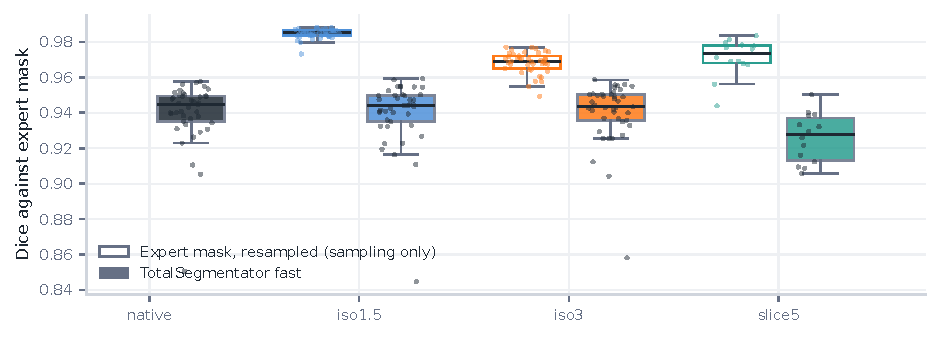
\includegraphics[width=\linewidth]{dice_by_resolution.pdf}
\caption{Dice by resolution level. Hollow boxes: the expert mask, resampled (sampling only). Filled boxes: TotalSegmentator fast run on the resampled CT. Points are scans.}
\label{f:dice}
\end{figure}
Sampling alone costs between 1.5 and 3 Dice points: the resampled expert mask scores 0.985, 0.968 and 0.971, with HD95 of 0.81, 1.20 and 2.37\,mm. TotalSegmentator scores Dice 0.940 at native, \lvl{iso1.5} and \lvl{iso3} alike, and its HD95 even falls slightly (3.18, 3.07, 3.03\,mm). With 5\,mm slices its Dice falls from 0.941 to 0.926 and its HD95 rises from 3.04 to 3.79\,mm on the same 14 scans (Table~\ref{t:mask}, Figure~\ref{f:dice}).

\subsection{Meshes against the reference surface}
\begin{table}[H]
\centering\small
\fitwidth{\begin{tabular}{lllrrrrrr}
\toprule
Source & Level & Config & ASSD (mm) & HD95 (mm) & NSD@1\,mm & Signed (mm) & Volume (\%) & Closed \\
\midrule
Expert mask & \texttt{native} & Canonical & 0.000 $\pm$ 0.000 & 0.00 $\pm$ 0.00 & 1.000 $\pm$ 0.000 & -0.000 $\pm$ 0.000 & -0.0 $\pm$ 0.0 & 98\% \\
Expert mask & \texttt{native} & Production & 0.234 $\pm$ 0.056 & 0.70 $\pm$ 0.17 & 0.996 $\pm$ 0.005 & -0.022 $\pm$ 0.013 & -0.3 $\pm$ 0.3 & 98\% \\
Expert mask & \texttt{iso1.5} & Canonical & 0.204 $\pm$ 0.017 & 0.61 $\pm$ 0.04 & 1.000 $\pm$ 0.000 & -0.003 $\pm$ 0.013 & -0.1 $\pm$ 0.2 & 98\% \\
Expert mask & \texttt{iso1.5} & Production & 0.374 $\pm$ 0.098 & 1.10 $\pm$ 0.31 & 0.940 $\pm$ 0.042 & -0.043 $\pm$ 0.025 & -0.7 $\pm$ 0.5 & 95\% \\
Expert mask & \texttt{iso3} & Canonical & 0.418 $\pm$ 0.030 & 1.18 $\pm$ 0.11 & 0.923 $\pm$ 0.020 & -0.039 $\pm$ 0.021 & -0.6 $\pm$ 0.4 & 98\% \\
Expert mask & \texttt{iso3} & Production & 0.517 $\pm$ 0.126 & 1.50 $\pm$ 0.36 & 0.860 $\pm$ 0.077 & -0.142 $\pm$ 0.039 & -2.0 $\pm$ 0.9 & 98\% \\
Expert mask & \texttt{slice5} & Canonical & 0.445 $\pm$ 0.079 & 1.46 $\pm$ 0.26 & 0.850 $\pm$ 0.045 & 0.053 $\pm$ 0.095 & 0.5 $\pm$ 1.2 & 100\% \\
Expert mask & \texttt{slice5} & Production & 0.425 $\pm$ 0.127 & 1.37 $\pm$ 0.32 & 0.877 $\pm$ 0.067 & 0.013 $\pm$ 0.097 & 0.1 $\pm$ 1.2 & 93\% \\
\midrule
TotalSegmentator fast & \texttt{native} & Canonical & 0.901 $\pm$ 0.197 & 3.15 $\pm$ 1.58 & 0.659 $\pm$ 0.051 & 0.261 $\pm$ 0.263 & 1.8 $\pm$ 3.4 & 98\% \\
TotalSegmentator fast & \texttt{native} & Production & 0.948 $\pm$ 0.218 & 3.03 $\pm$ 1.65 & 0.638 $\pm$ 0.058 & 0.221 $\pm$ 0.251 & 1.4 $\pm$ 3.4 & 66\% \\
TotalSegmentator fast & \texttt{iso1.5} & Canonical & 0.905 $\pm$ 0.223 & 3.02 $\pm$ 1.65 & 0.647 $\pm$ 0.060 & 0.157 $\pm$ 0.270 & 0.7 $\pm$ 3.7 & 98\% \\
TotalSegmentator fast & \texttt{iso1.5} & Production & 0.958 $\pm$ 0.255 & 3.03 $\pm$ 1.72 & 0.636 $\pm$ 0.075 & 0.099 $\pm$ 0.255 & 0.2 $\pm$ 3.6 & 90\% \\
TotalSegmentator fast & \texttt{iso3} & Canonical & 0.907 $\pm$ 0.206 & 2.95 $\pm$ 1.56 & 0.652 $\pm$ 0.061 & 0.180 $\pm$ 0.267 & 1.1 $\pm$ 3.5 & 98\% \\
TotalSegmentator fast & \texttt{iso3} & Production & 0.914 $\pm$ 0.247 & 2.84 $\pm$ 1.51 & 0.659 $\pm$ 0.084 & 0.038 $\pm$ 0.248 & -0.5 $\pm$ 3.4 & 95\% \\
TotalSegmentator fast & \texttt{slice5} & Canonical & 1.079 $\pm$ 0.152 & 3.51 $\pm$ 2.14 & 0.578 $\pm$ 0.046 & 0.123 $\pm$ 0.366 & -0.3 $\pm$ 3.7 & 100\% \\
TotalSegmentator fast & \texttt{slice5} & Production & 1.048 $\pm$ 0.169 & 3.35 $\pm$ 2.14 & 0.588 $\pm$ 0.058 & 0.075 $\pm$ 0.358 & -0.6 $\pm$ 3.7 & 50\% \\
\bottomrule
\end{tabular}
}
\caption{Mesh-level error against the reference surface (the canonical expert mesh at native resolution). \emph{Signed}: mean signed distance; negative means shrinkage. \emph{Closed}: share of meshes with no boundary and no non-manifold edges.}
\label{t:mesh}
\end{table}
\begin{figure}[H]
\centering
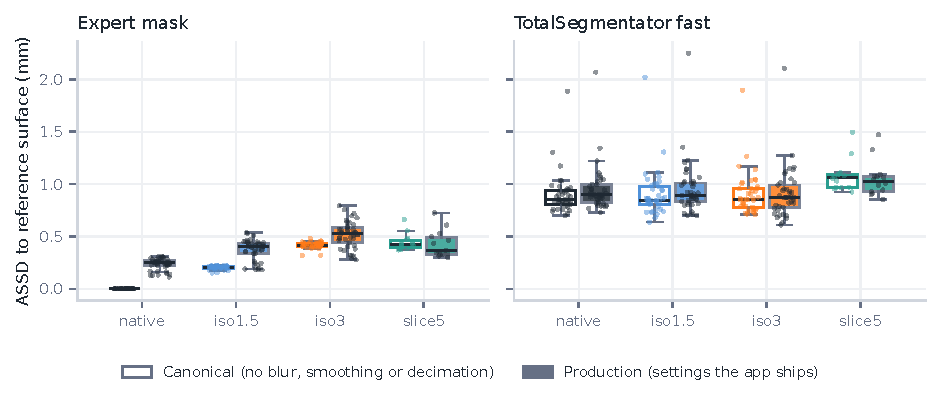
\includegraphics[width=\linewidth]{assd_by_resolution.pdf}
\caption{ASSD to the reference surface by level. Hollow boxes: canonical reconstruction. Filled boxes: the app's production settings. Points are scans.}
\label{f:assd}
\end{figure}
Two regimes appear (Table~\ref{t:mesh}, Figure~\ref{f:assd}).

\begin{itemize}
\item \textbf{The expert mask's error tracks resolution.} The canonical expert mesh moves 0.204, 0.418 and 0.445\,mm from the reference at \lvl{iso1.5}, \lvl{iso3} and \lvl{slice5}. Production settings add to this on finer grids: 0.234\,mm at native, 0.374\,mm at \lvl{iso1.5} and 0.517\,mm at \lvl{iso3}.
\item \textbf{TotalSegmentator's error is flat until the slices thicken.} Its canonical error is 0.90--0.91\,mm at native, \lvl{iso1.5} and \lvl{iso3}, and 1.08\,mm at \lvl{slice5}. At every coarse level its canonical error is 2.2--4.4 times the expert mask's: segmentation, not sampling, sets the error budget.
\end{itemize}

\subsection{Paired effect of each level}
\begin{table}[H]
\centering\small
\fitwidth{\begin{tabular}{lllrrrrrr}
\toprule
Source & Config & Level & $n$ & At native & At level & Difference [95\% CI] & Median ratio & Wilcoxon $p$ \\
\midrule
Expert mask & Canonical & \texttt{iso1.5} & 41 & 0.000 & 0.204 & +0.204 [+0.198, +0.209] & -- & $<$0.001 \\
Expert mask & Canonical & \texttt{iso3} & 41 & 0.000 & 0.418 & +0.418 [+0.408, +0.426] & -- & $<$0.001 \\
Expert mask & Canonical & \texttt{slice5} & 14 & 0.000 & 0.445 & +0.445 [+0.411, +0.490] & -- & $<$0.001 \\
Expert mask & Production & \texttt{iso1.5} & 41 & 0.234 & 0.374 & +0.140 [+0.125, +0.155] & 1.59$\times$ & $<$0.001 \\
Expert mask & Production & \texttt{iso3} & 41 & 0.234 & 0.517 & +0.283 [+0.258, +0.308] & 2.25$\times$ & $<$0.001 \\
Expert mask & Production & \texttt{slice5} & 14 & 0.176 & 0.425 & +0.248 [+0.211, +0.295] & 2.45$\times$ & $<$0.001 \\
\midrule
TotalSegmentator fast & Canonical & \texttt{iso1.5} & 41 & 0.901 & 0.905 & +0.004 [-0.019, +0.026] & 1.00$\times$ & 0.635 \\
TotalSegmentator fast & Canonical & \texttt{iso3} & 41 & 0.901 & 0.907 & +0.006 [-0.006, +0.019] & 1.00$\times$ & 0.663 \\
TotalSegmentator fast & Canonical & \texttt{slice5} & 14 & 0.890 & 1.079 & +0.188 [+0.150, +0.229] & 1.19$\times$ & $<$0.001 \\
TotalSegmentator fast & Production & \texttt{iso1.5} & 41 & 0.948 & 0.958 & +0.010 [-0.017, +0.037] & 1.01$\times$ & 0.411 \\
TotalSegmentator fast & Production & \texttt{iso3} & 41 & 0.948 & 0.914 & -0.034 [-0.055, -0.013] & 0.96$\times$ & 0.003 \\
TotalSegmentator fast & Production & \texttt{slice5} & 14 & 0.915 & 1.048 & +0.134 [+0.098, +0.171] & 1.13$\times$ & $<$0.001 \\
\bottomrule
\end{tabular}
}
\caption{Change in ASSD (mm) at each level against native, paired by scan, over resampled scans only. CI: 95\% bootstrap interval of the mean difference. The canonical expert mesh at native \emph{is} the reference, so it has no ratio.}
\label{t:paired}
\end{table}
For the expert mask every level is a clear, significant increase (Table~\ref{t:paired}). For TotalSegmentator, the canonical meshes do not change at \lvl{iso1.5} or \lvl{iso3}: the differences are $+0.004$ and $+0.006$\,mm, and both confidence intervals include zero. With 5\,mm slices they worsen by 0.188\,mm.

The production meshes behave differently. At \lvl{iso3} they \emph{improve} by 0.034\,mm [0.013, 0.055] ($p=0.003$), and the share of closed meshes rises from 66\% to 95\%. A likely reason is that TotalSegmentator fast predicts at 3\,mm and returns its mask on the input grid. At native resolution the mask therefore carries 3\,mm steps sampled on a fine grid, which the production blur of 0.6 native voxels cannot smooth away. The resulting large mesh (median 19{,}520 faces against 2{,}600) then loses topology under 60\% decimation.

\subsection{A sampling law for real anatomy}
\begin{figure}[H]
\centering
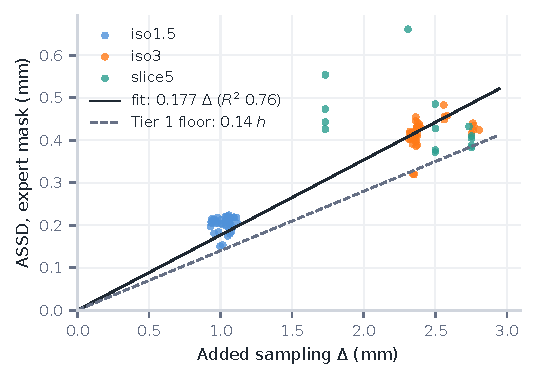
\includegraphics[width=0.62\linewidth]{sampling_floor.pdf}
\caption{Canonical expert-mask ASSD against the sampling added by coarsening, $\Delta=\sqrt{\tfrac13\sum_a (s_a'^2-s_a^2)}$, for every resampled scan and level. Solid line: least-squares fit through the origin. Dashed line: the Tier~1 floor, $0.14\,h$, for an isotropic grid $h$ against an exact surface.}
\label{f:floor}
\end{figure}
Neither the coarse grid's geometric-mean spacing nor its largest spacing predicts the expert mask's error ($R^2<0$ for a fit through the origin). What matters is how much each axis was coarsened \emph{relative to native}: the reference already contains the native sampling. Sampling blur adds in quadrature, so the natural measure is $\Delta=\sqrt{\tfrac13\sum_a (s_a'^2-s_a^2)}$, which equals $h$ when an isotropic grid of spacing $h$ replaces an infinitely fine one.

Against $\Delta$, the three levels fall on one line: $\text{ASSD}=0.177\,\Delta$ ($R^2=0.76$, $r=0.89$; Figure~\ref{f:floor}). The ratio is nearly the same at each level: 0.199, 0.172 and 0.199 for \lvl{iso1.5}, \lvl{iso3} and \lvl{slice5}. This agrees in magnitude with Tier~1's $0.14\,h$, measured against exact phantom surfaces. A practical reading: \emph{every millimetre of added sampling costs about 0.18\,mm of surface accuracy}, before any segmentation error.

\subsection{Variance attribution}
\begin{table}[H]
\centering\small
\begin{tabular}{lrrrrr}
\toprule
& \multicolumn{3}{c}{ASSD (mm)} & \multicolumn{2}{c}{log ASSD} \\
\cmidrule(lr){2-4}\cmidrule(lr){5-6}
Factor & All & Expert & TotalSeg. & Expert (coarse) & TotalSeg. \\
\midrule
Mask source & 71.3\% & -- & -- & -- & -- \\
Resolution level & 2.8\% & 50.5\% & 2.7\% & 34.5\% & 4.3\% \\
Blur & 0.0\% & 0.9\% & 0.0\% & 0.3\% & 0.0\% \\
Taubin iterations & 1.1\% & 16.0\% & 0.4\% & 14.5\% & 0.5\% \\
Decimation & 0.0\% & 0.4\% & 0.0\% & 0.6\% & 0.0\% \\
Case (patient) & 9.7\% & 10.3\% & 89.5\% & 19.5\% & 84.0\% \\
\midrule
Interactions + residual & 15.1\% & 21.9\% & 7.4\% & 30.6\% & 11.2\% \\
\bottomrule
\end{tabular}

\caption{Main-effect share of variance ($\eta^2$) across the 48 grid configurations. ASSD in millimetres is primary. Log-ASSD is shown only where it is well defined: the canonical expert mesh at native reproduces the reference exactly (ASSD $=0$), and decimating it often changes nothing (ASSD $\approx10^{-15}$), so the log scale is dominated by those exact zeros.}
\label{t:variance}
\end{table}
\begin{figure}[H]
\centering
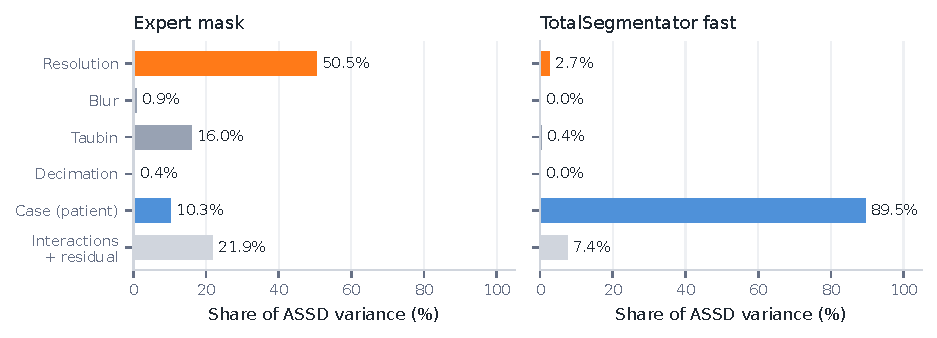
\includegraphics[width=\linewidth]{variance_shares.pdf}
\caption{Share of ASSD variance by factor, for the expert mask (left) and TotalSegmentator (right).}
\label{f:variance}
\end{figure}
Across all meshes, the mask source alone explains 71.3\% of ASSD variance (Table~\ref{t:variance}). Within each source the picture splits (Figure~\ref{f:variance}).

\begin{itemize}
\item \textbf{Expert mask:} resolution 50.5\%, Taubin smoothing 16.0\%, case 10.3\%, blur 0.9\% and decimation 0.4\%. This mirrors Tier~1, where spacing explained 68.6\%.
\item \textbf{TotalSegmentator:} case 89.5\% and resolution 2.7\%. Every reconstruction setting is below 0.5\%.
\end{itemize}

The log scale, where defined, tells the same story (TotalSegmentator: case 84.0\%; expert mask below native: resolution 34.5\%, case 19.5\%, Taubin 14.5\%).

\subsection{Smoothing and blur reverse sign with slice thickness}
\begin{table}[H]
\centering\small
\begin{minipage}[t]{0.49\linewidth}\centering
\fitwidth{\begin{tabular}{llrrrr}
\toprule
Source & Level & 0 it. & 10 it. & 30 it. & 60 it. \\
\midrule
Expert mask & \texttt{native} & 0.000 & 0.046 & 0.215 & 0.306 \\
Expert mask & \texttt{iso1.5} & 0.204 & 0.227 & 0.356 & 0.421 \\
Expert mask & \texttt{iso3} & 0.418 & 0.422 & 0.475 & 0.537 \\
Expert mask & \texttt{slice5} & 0.445 & 0.439 & 0.425 & 0.427 \\
\midrule
TotalSegmentator fast & \texttt{native} & 0.901 & 0.911 & 0.961 & 0.978 \\
TotalSegmentator fast & \texttt{iso1.5} & 0.905 & 0.926 & 0.975 & 0.975 \\
TotalSegmentator fast & \texttt{iso3} & 0.907 & 0.920 & 0.929 & 0.919 \\
TotalSegmentator fast & \texttt{slice5} & 1.079 & 1.074 & 1.062 & 1.047 \\
\bottomrule
\end{tabular}
}\\[2pt]
{\footnotesize (a) Taubin iterations; no blur, no decimation.}
\end{minipage}\hfill
\begin{minipage}[t]{0.49\linewidth}\centering
\fitwidth{\begin{tabular}{llrrr}
\toprule
Source & Level & 0\,mm & 0.5\,mm & 1\,mm \\
\midrule
Expert mask & \texttt{native} & 0.000 & 0.075 & 0.186 \\
Expert mask & \texttt{iso1.5} & 0.204 & 0.206 & 0.260 \\
Expert mask & \texttt{iso3} & 0.418 & 0.417 & 0.419 \\
Expert mask & \texttt{slice5} & 0.445 & 0.418 & 0.394 \\
\midrule
TotalSegmentator fast & \texttt{native} & 0.901 & 0.916 & 0.932 \\
TotalSegmentator fast & \texttt{iso1.5} & 0.905 & 0.907 & 0.931 \\
TotalSegmentator fast & \texttt{iso3} & 0.907 & 0.909 & 0.909 \\
TotalSegmentator fast & \texttt{slice5} & 1.079 & 1.070 & 1.054 \\
\bottomrule
\end{tabular}
}\\[2pt]
{\footnotesize (b) Blur; no smoothing, no decimation.}
\end{minipage}
\caption{Mean ASSD (mm) by smoothing and by blur at each level.}
\label{t:smooth}
\end{table}
\begin{figure}[H]
\centering
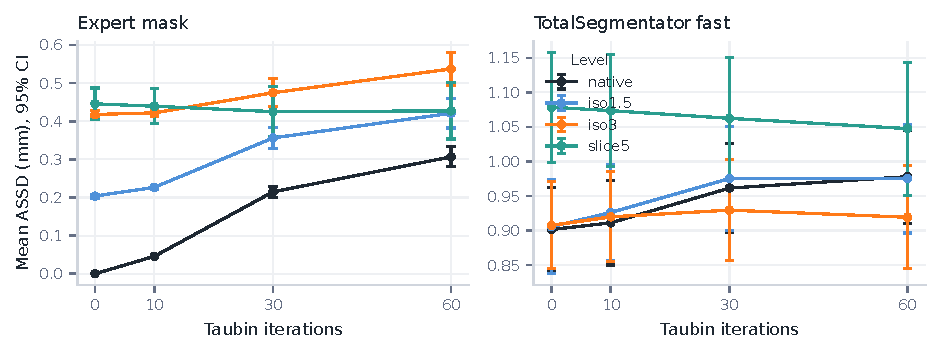
\includegraphics[width=\linewidth]{taubin_by_resolution.pdf}
\caption{Mean ASSD against Taubin iterations at each level (no blur, no decimation), with 95\% confidence intervals across scans.}
\label{f:taubin}
\end{figure}
On fine grids, smoothing moves meshes away from the reference. With 60 iterations the expert mesh moves 0.306\,mm at native, and TotalSegmentator's error rises from 0.901 to 0.978\,mm. With 5\,mm slices the sign reverses: 60 iterations bring the expert mesh from 0.445 to 0.427\,mm and TotalSegmentator from 1.079 to 1.047\,mm. Blur behaves the same way: 1\,mm of blur moves the native expert mesh 0.186\,mm but brings the \lvl{slice5} mesh from 0.445 to 0.394\,mm (Table~\ref{t:smooth}, Figure~\ref{f:taubin}).

On a compact organ, smoothing helps once the sampling staircase is large (5\,mm steps) and otherwise pulls the mesh off the reference. Two caveats apply:
\begin{itemize}
\item At native resolution the reference \emph{is} the unsmoothed staircase, so part of that ``error'' is departure from the staircase itself (Section~\ref{s:floor}).
\item Tier~1 also saw smoothing change sign with spacing, but in the opposite direction: it hurt at coarse spacing. That was driven by a thin 2\,mm-radius capsule, which smoothing shrinks. For thin structures shrinkage may win over staircase removal, which CT-ORG's bone will test.
\end{itemize}

\subsection{Systematic bias}
\begin{figure}[H]
\centering
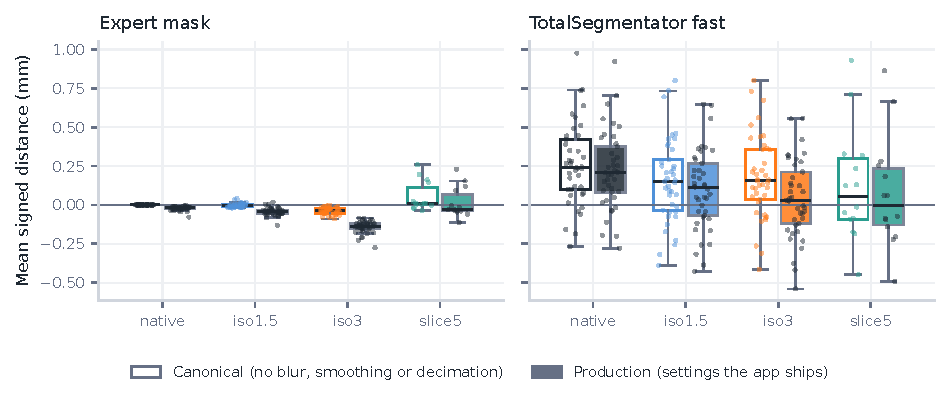
\includegraphics[width=\linewidth]{signed_by_resolution.pdf}
\caption{Mean signed distance to the reference surface by level. Negative values mean the mesh lies inside the reference (shrinkage); positive values mean it lies outside (expansion).}
\label{f:signed}
\end{figure}
The two sources are biased in opposite directions (Figure~\ref{f:signed}, Table~\ref{t:mesh}).

\begin{itemize}
\item \textbf{The app's settings shrink the expert mesh, more so on coarse grids.} The mean signed distance is $-0.022$\,mm at native and $-0.142$\,mm at \lvl{iso3}, with volume errors of $-0.3\%$ and $-2.0\%$. The production blur is set in voxels, so on a 3\,mm grid its 0.6 voxels become 1.8\,mm, enough to erode a convex organ.
\item \textbf{TotalSegmentator over-segments slightly.} Its canonical meshes lie 0.26\,mm outside the expert surface at native (volume $+1.8\%$) and 0.12--0.18\,mm outside at the coarser levels. The production settings largely cancel this offset at \lvl{iso3} (0.038\,mm): the shrinkage of the reconstruction offsets the expansion of the segmentation.
\end{itemize}

\subsection{Topology}
\begin{table}[H]
\centering\small
\begin{tabular}{llrrrr}
\toprule
Source & Level & 0 & 0.25 & 0.5 & 0.75 \\
\midrule
Expert mask & \texttt{native} & 98\% & 96\% & 90\% & 68\% \\
Expert mask & \texttt{iso1.5} & 98\% & 95\% & 92\% & 75\% \\
Expert mask & \texttt{iso3} & 98\% & 97\% & 93\% & 79\% \\
Expert mask & \texttt{slice5} & 100\% & 100\% & 93\% & 71\% \\
\midrule
TotalSegmentator fast & \texttt{native} & 98\% & 97\% & 93\% & 57\% \\
TotalSegmentator fast & \texttt{iso1.5} & 98\% & 98\% & 93\% & 63\% \\
TotalSegmentator fast & \texttt{iso3} & 98\% & 95\% & 94\% & 83\% \\
TotalSegmentator fast & \texttt{slice5} & 100\% & 99\% & 95\% & 58\% \\
\bottomrule
\end{tabular}

\caption{Share of grid meshes that are closed and manifold, by decimation (fraction of faces removed). One scan (2.4\%) is open at the field of view at every setting, which caps most columns at 98\%.}
\label{t:topology}
\end{table}
\begin{figure}[H]
\centering
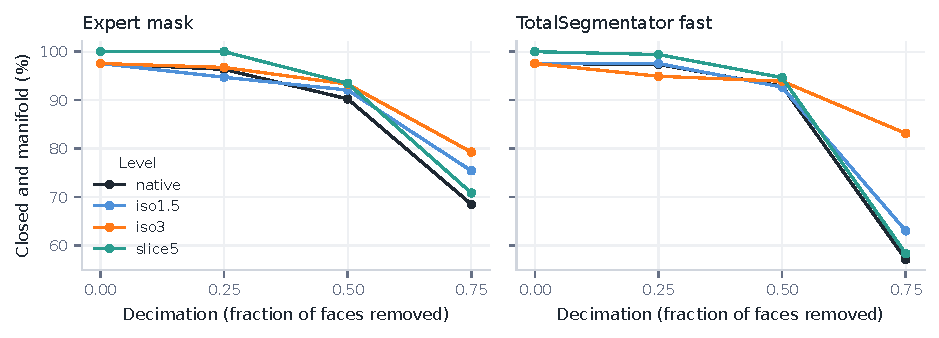
\includegraphics[width=\linewidth]{topology_by_decimation.pdf}
\caption{Closed and manifold meshes against decimation, by level.}
\label{f:topology}
\end{figure}
Decimation explains almost none of the ASSD variance (0.0--0.4\%), but it drives topology (Table~\ref{t:topology}, Figure~\ref{f:topology}).

\begin{itemize}
\item \textbf{Geometry is largely spared on unsmoothed meshes.} Decimating the canonical expert mesh by 25\% or 50\% leaves its surface exactly unchanged in 39 and 34 of 41 scans (ASSD below $10^{-6}$\,mm). Marching cubes on a binary mask produces large coplanar patches, and decimation first merges those.
\item \textbf{Topology breaks}, even though VTK's decimation runs in its topology-preserving mode. At 75\%, only 57--83\% of meshes remain closed. TotalSegmentator meshes on the native grid fare worst (57\%) and those on the 3\,mm grid best (83\%).
\item \textbf{The one remaining open reference is a property of the data.} In scan \texttt{spleen\_26} the expert spleen touches the first slice, so every mesh of it is open where the field of view cuts it (380 boundary edges in the reference). This accounts for the $\approx$2\% of non-closed canonical meshes seen in both runs.
\end{itemize}

\subsection{Numerical reproducibility}
\begin{table}[H]
\centering\small
\begin{tabular}{llrrrr}
\toprule
Source & Meshes & Rows & Max $|\Delta|$ ASSD (mm) & Median $|\Delta|$ (mm) & Topology flips \\
\midrule
Expert mask & no decimation & 492 & 0.0e+00 & 0.0e+00 & 0 (0.0\%) \\
Expert mask & decimated & 1517 & 0.0e+00 & 0.0e+00 & 0 (0.0\%) \\
TotalSegmentator fast & no decimation & 492 & 4.0e-04 & 2.5e-05 & 0 (0.0\%) \\
TotalSegmentator fast & decimated & 1517 & 1.6e-02 & 1.0e-04 & 12 (0.8\%) \\
\bottomrule
\end{tabular}

\caption{Native-resolution rows of this run against the earlier native-only run (same seed). $|\Delta|$: absolute difference in ASSD.}
\label{t:repro}
\end{table}
Adding the resolution factor changed how masks are cropped: each mask is now cropped on its own grid instead of jointly with the expert mask. The native rows were compared with the earlier run to confirm nothing else changed (Table~\ref{t:repro}).

\begin{itemize}
\item \textbf{Expert-mask rows reproduce exactly} (2{,}009 rows, zero difference), because their crop did not change.
\item \textbf{TotalSegmentator rows differ only at floating-point level.} Marching cubes returns float32 vertices, so a 2-voxel shift of the crop origin changes their last bit: at most $1.5\times10^{-5}$\,mm, measured directly. Without decimation this leaves ASSD within $4\times10^{-4}$\,mm. Decimation's greedy choices amplify it to at most 0.016\,mm (median $1\times10^{-4}$), and it flips 12 of 1{,}517 decimated meshes (0.8\%) between closed and open.
\end{itemize}

Decimated topology is therefore not stable at machine precision, and topology rates should be read with about $\pm1$ percentage point of numerical noise.

\section{Discussion}

\subsection{What this means for RQ1}
The results separate two regimes.

\begin{itemize}
\item \textbf{When the segmentation is right (the expert mask)}, acquisition resolution is the leading source of surface error, as in Tier~1. It explains 50.5\% of variance and follows $\text{ASSD}\approx0.18\,\Delta$. Smoothing is second (16.0\%).
\item \textbf{When a real engine segments}, the error is set by the engine and by the patient: 89.5\% of variance is case-to-case. Resolution matters only through thick slices, and reconstruction settings barely register.
\end{itemize}

TotalSegmentator fast is insensitive to in-plane resolution because it already works at 3\,mm. Its full-resolution model (1.5\,mm) may behave differently, and that is the next comparison.

For the stage-wise attribution in RQ1, the ranking for automatic pipelines is: segmentation engine and case $\gg$ thick slices $>$ smoothing $>$ blur $\approx$ decimation (for geometry). Decimation, however, dominates topology.

The case-driven error is also the premise of \textbf{RQ2}. If 89.5\% of an engine's error is patient-specific, a ground-truth-free reliability estimate has to read the case (image and mask features), not the pipeline settings. And because coarser grids cost TotalSegmentator fast nothing, \textbf{RQ3}'s cost-constrained selection has real room to save compute.

\subsection{How to read errors near the reference}\label{s:floor}
The reference surface is a reference standard, not the truth. It is built at native resolution and carries that resolution's own sampling error. By Tier~1's $0.14\,h$ (or this report's $0.177\,\Delta$, taking the native grid against an ideal one), that floor is a median 0.41 (0.52)\,mm for the 24 scans with 5\,mm slices and 0.17 (0.21)\,mm for scans with slices of 2.5\,mm or less.

So the 0.234\,mm that production settings add to the expert mask at native resolution, and the movement caused by smoothing on fine grids, are \emph{departures from the reference staircase}. They are below its own resolution and cannot be called anatomical error. TotalSegmentator's 0.9\,mm sits well above the floor, so the engine-level conclusions are robust. The Tier~1 phantoms remain the only place where reconstruction error is measured against an exact surface.

\subsection{Candidate changes to MEDSYS}
These are candidates only, not yet made. Each should be confirmed on CT-ORG before the app changes.

\begin{enumerate}
\item \textbf{Mesh TotalSegmentator fast output on a 3\,mm grid.} This gave 0.034\,mm lower ASSD, 95\% instead of 66\% closed meshes and 7.5$\times$ fewer faces. Any gain in viewer quality comes at no accuracy cost.
\item \textbf{Specify the mask blur in millimetres, not voxels.} The voxel-based blur shrinks meshes as grids coarsen ($-2.0\%$ volume at 3\,mm).
\item \textbf{Treat decimation as a topology risk.} Use lower reduction, or check and repair closedness after decimating, wherever closed meshes matter (volume measurement, 3D printing).
\item \textbf{Flag scans whose organ touches the field of view.} The mesh will be open there regardless of settings.
\end{enumerate}

\subsection{Limitations}
\begin{itemize}
\item \textbf{One structure, one dataset.} The spleen is a large, compact organ. Thin or branching structures (vessels, bone) and high-contrast ones (lungs) may respond differently to resolution.
\item \textbf{Simulated, not real, coarser acquisitions.} Resampling with a Gaussian aperture approximates a coarser slice profile but not reconstruction kernels, noise or partial-volume effects at acquisition time.
\item \textbf{Only 14 scans at \lvl{slice5}}, since most scans already had 5\,mm slices. Its effects have wider intervals.
\item \textbf{A single expert per scan.} Inter-rater variability, which bounds any reference standard, is not measured.
\item \textbf{Descriptive attribution only.} The analysis uses main-effect $\eta^2$ on an unbalanced design (the \lvl{slice5} level is smaller); the planned mixed-effects model and Sobol indices are still to come.
\item \textbf{TotalSegmentator fast only.} The full 1.5\,mm model was not run. Engine masks at native resolution were reused from the earlier run rather than re-segmented, so GPU non-determinism was not measured.
\item \textbf{Code at run time.} The run recorded commit \texttt{46c9b8b} with uncommitted changes. Those changes are the resolution factor described here, committed together with this report.
\end{itemize}

\section{Next steps}
\begin{enumerate}
\item \textbf{CT-ORG} (liver; lungs and bone in the hand-labelled cases 0--20), with the classical engine alongside TotalSegmentator. Thinner slices there will give \lvl{slice5} a full sample.
\item \textbf{TotalSegmentator full (1.5\,mm)}, the canonical engine in the study design. Is a finer model sensitive to resolution where the fast model is not?
\item \textbf{Formal attribution:} a mixed-effects model with case as a random effect, plus Sobol indices for the continuous reconstruction settings.
\item \textbf{Validate the candidate app changes} above on CT-ORG before adopting them.
\item \textbf{RQ2 groundwork:} the case-level features (image quality, mask shape, model confidence) that could predict the 89.5\% of engine error that is patient-specific.
\end{enumerate}

\appendix
\section{Reproducing this report}
\begin{small}
\begin{verbatim}
# 1. Segment and score (GPU used for TotalSegmentator if available)
python -m research.tier2 --dataset msd_spleen --data data/msd/Task09_Spleen \
       --preset full --workers 5
# 2. Tables, figures and numbers.json for this report
python -m research.tier2_report output/research/tier2/20261004-214129_msd_spleen_full \
       --out docs/tier2-report \
       --baseline output/research/tier2/20261003-093356_msd_spleen_full
# 3. Compile (twice, for references)
cd docs/tier2-report && pdflatex tier2-resolution-report.tex
\end{verbatim}
\end{small}

\textbf{Run:} \texttt{output/research/tier2/20261004-214129\_msd\_spleen\_full}, seed 2026, 20{,}000 surface samples per side, NSD tolerance 1\,mm. \textbf{Software:} Python 3.14.4, NumPy 2.4.4, SciPy 1.17.1, scikit-image 0.26.0, PyVista 0.48.4, VTK 9.6.2, nibabel 5.4.2, PyTorch 2.12.0 (CUDA 13.0), TotalSegmentator 2.13.0. \textbf{Hardware:} Windows~11, 6-core CPU, NVIDIA GeForce RTX 5080 (16\,GB). \textbf{Data:} MSD Task09 Spleen, 41 training scans (CC-BY-SA 4.0); the scans and labels are not redistributed with this report.

\section*{References}
{\small
\begin{enumerate}[label={[\arabic*]},leftmargin=*,itemsep=1pt]
\item\label{r:msd} M.~Antonelli \emph{et al.}, ``The Medical Segmentation Decathlon,'' \emph{Nature Communications}, 13, 4128, 2022.
\item\label{r:tspaper} J.~Wasserthal \emph{et al.}, ``TotalSegmentator: robust segmentation of 104 anatomic structures in CT images,'' \emph{Radiology: Artificial Intelligence}, 2023. \href{https://doi.org/10.1148/ryai.230024}{doi:10.1148/ryai.230024}
\item\label{r:nnunet} F.~Isensee \emph{et al.}, ``nnU-Net: a self-configuring method for deep learning-based biomedical image segmentation,'' \emph{Nature Methods}, 18, 203--211, 2021.
\item\label{r:lewiner} T.~Lewiner, H.~Lopes, A.~W.~Vieira and G.~Tavares, ``Efficient implementation of Marching Cubes' cases with topological guarantees,'' \emph{Journal of Graphics Tools}, 8(2), 2003.
\item\label{r:taubin} G.~Taubin, ``A signal processing approach to fair surface design,'' \emph{Proc.\ SIGGRAPH}, 1995.
\item\label{r:schroeder} W.~J.~Schroeder, J.~A.~Zarge and W.~E.~Lorensen, ``Decimation of triangle meshes,'' \emph{Proc.\ SIGGRAPH}, 1992.
\item\label{r:skimage} S.~van der Walt \emph{et al.}, ``scikit-image: image processing in Python,'' \emph{PeerJ}, 2:e453, 2014.
\item\label{r:nsd} S.~Nikolov \emph{et al.}, ``Clinically applicable segmentation of head and neck anatomy for radiotherapy: deep learning algorithm development and validation study,'' \emph{Journal of Medical Internet Research}, 23(7), 2021.
\item\label{r:montgomery} D.~C.~Montgomery, \emph{Design and Analysis of Experiments}, Wiley.
\item\label{r:saltelli} A.~Saltelli \emph{et al.}, \emph{Global Sensitivity Analysis: The Primer}, Wiley, 2008.
\end{enumerate}
}

\end{document}
